\documentclass{article}
\usepackage{graphicx}
\usepackage{float}
\usepackage{mathtools}

\title{ELEC 302-81\\ Lab 4\\ Transformers in Three Phase Circuits}
\date{\today} 

\begin{document}

\maketitle

\begin{center}
  \begin{tabular}{lr}
    Date Performed: & February 11, 2013 \\
    Partners: & Rawley Dent \\
              & Charles Pittman \\
    Instructor: & Dr. Weatherford
  \end{tabular}
\end{center}

\pagebreak

\setlength\parindent{0pt} 

\section{Purpose of Experiment}

The purpose of this experiment was to observe the basic principals of balanced
three-phase transformer circuits. Y-Y and Y-$\Delta$ connected transformer banks 
were constructed separately to observe the differences, particularly in their 
respective loads. Primary and secondary voltages, currents, and powers were first 
calculated theoretically. Experimental values were then measured to compare. 

\section{Procedure}

\subsection{EMS Workstation Set-up}

At the Lab-Volt EMS workstation, the DAI 24V supply was turned on, and the DAI USB
connector was connected between the EMS workstation and the {PC}. On the LVDAM
EMS application software, the metering windows for E$_1$, E$_2$, I$_1$, I$_2$, 
P$_1$, 3 phase power, E$_3$, I$_3$, and E$_1$ + E$_2$ + E$_3$ were opened. 
Under \emph{Options} -> \emph{Acquistion Settings}, the \emph{Sample Window} dialog box 
was set to extended, and under \emph{View} -> the continuous refresh option was checked.

\subsection{The Three Phase Source}

\label{part1} The circuit represented by Figure~\ref{fig:circuit_01} was constructed.
The main power switch was set ON and the voltage supply was adjusted to 120-V line-to-
line. Both the installed analog EMS voltmeter and the metering window were monitored
for proper indications. The line voltages were then measured and recorded. These values 
are shown in Table~\ref{tab:3phase_source}. The main power switch was set OFF and the 
voltage supply fully CCW. The circuit represented by Figure~\ref{fig:circuit_02}
was constructed. The main power switch was set ON and the voltage supply was adjusted 
to read 120-V line-to-line. The installed analog EMS voltmeter was used for this since 
the 120-V were to be measured across voltage sources 4-5 only. The phase voltages were
then measured and recorded. These values are shown in Table~\ref{tab:3phase_source}.  
The main power switch was set OFF and the voltage supply fully CCW.

\subsection{Y--Y Connected Transformer}

\label{part2} The circuit shown in Figure~\ref{fig:circuit_03} was constructed. The 
Y-connected load was 600 + j300 $\Omega$. The main power switch was turned on and the 
voltage control knob was adjusted to 120-V line-to-line. The analog EMS voltmeter and 
the metering window were both monitored for correct voltage. The values for primary and 
secondary line voltage, primary and secondary line current, and primary input power were
measured and recorded. A Fluke multimeter was used to measure the RMS voltage across the 
load. This load voltage was labeled as $E_4$. These values are shown in Table~\ref{tab:results}.  
The main power switch was set OFF and the voltage control knob fully CCW.

\subsection{Y--$\Delta$ Connected Transformer}

\label{part3} The circuit shown in Figure~\ref{fig:circuit_04} was then constructed. 
The Y-connected load was 600 + j300 $\Omega$. The main power switch was turned on and the 
voltage control knob was adjusted to 120-V line-to-line. The analog EMS voltmeter and 
the metering window were both monitored for correct voltage. The values for primary and 
secondary line voltage, primary and secondary line current, and primary input power were
measured and recorded. A Fluke multimeter was used to measure the RMS voltage across the 
load. This load voltage was labeled as $E_4$. These values are shown in Table~\ref{tab:results}.  
The main power switch was set OFF and the voltage control knob fully CCW.

\section{Results}
\subsection{The Three Phase Source}
\begin{table}[H]
  \centering
  \begin{tabular}{*{5}{c}}
    & \textbf{$E_1$} & \textbf{$E_2$} & \textbf{$E_3$} & \textbf{$E_1$+$E_2$+$E_3$} \\
    
    \hline
    
    \textbf{$V_{LL}$} & 120.4 & 117.1 & 116.3 & 0.998 \\
    \textbf{$V_{phase}$} & 69.77 & 64.56 & 69.01 & 5.15 \\
  \end{tabular}
  \caption{Measured line and phase voltages for Part 1}
  \label{tab:3phase_source}
\end{table}

\begin{table}[H]
  \centering
  \begin{tabular}{*{7}{c}}
    & \multicolumn{2}{c}{\textbf{Primary}} &
    \multicolumn{2}{c}{\textbf{Secondary}} & \textbf{3phase} & \textbf{Load} \\

    \textbf{Case} & \textbf{Voltage} & \textbf{Current} & \textbf{Voltage} &
    \textbf{Current} & \textbf{Input Power} & \textbf{Voltage} \\

    & $E_1$ V & $I_1$ A & $E_3$ V & $I_3$ A & $B$ W & $E_4$ V \\

    \hline
    Y--Y        & 121.2 & 0.112 & 119.5 & 0.097 & 19.8 & 58.4 \\
    Y--$\Delta$ & 120.1 & 0.151 & 68.4 & 0.055 & 4.7 & 32.4 \\
  \end{tabular}
  \caption{Measured Values}
  \label{tab:results}
\end{table}

\begin{table}[H]
  \centering
  \begin{tabular}{*{6}{c}}

    & \multicolumn{2}{c}{\textbf{Primary}}
    & \multicolumn{2}{c}{\textbf{Secondary}} & \textbf{Load} \\

    \textbf{Case} & \textbf{Line} & \textbf{Phase} & \textbf{Line} &
    \textbf{Phase} & \textbf{Phase} \\

    & V & V & V & V & V \\
    \hline

    Y--Y        & 120 & 69.3 & 120 & 11 & 69.3 \\
    Y--$\Delta$ & 120 & 69.3 & 69.3 & 11 & 40 \\
  \end{tabular}
  \caption{Computed Voltages}
  \label{tab:volt_comp}
\end{table}

\begin{table}[H]
  \centering
  \begin{tabular}{*{6}{c}}
    & \multicolumn{2}{c}{\textbf{Primary}}
    & \multicolumn{2}{c}{\textbf{Secondary}} & \textbf{Load} \\

    \textbf{Case} & \textbf{Line} & \textbf{Phase} & \textbf{Line} &
    \textbf{Phase} & \textbf{Phase} \\

    & A & A & A & A & A \\
    \hline

    Y--Y        & 0.1033 & 0.1033 & 0.1033 & 0.1033 & 0.1033 \\
    Y--$\Delta$ & 0.0596 & 0.0596 & 0.0344 & 0.0344 & 0.0344 \\
  \end{tabular}
  \caption{Computed Currents}
  \label{tab:curr_comp}
\end{table}

\begin{table}[H]
  \centering
  \begin{tabular}{*{4}{c}}
    \textbf{Case} & \textbf{Primary} & \textbf{Secondary} & \textbf{Load} \\

    & \textbf{Power} & \textbf{Power} & \textbf{Power} \\

    & W & W & W \\
    \hline

    Y--Y        & 19.20 & 19.20 & 19.2 \\
    Y--$\Delta$ & 6.40 & 6.4 & 6.4 \\
  \end{tabular}
  \caption{Computed Powers}
  \label{tab:pow_comp}
\end{table}

\begin{table}[H]
  \centering
  \begin{tabular}{*{7}{c}}
    & \multicolumn{2}{c}{\textbf{Primary}} &
    \multicolumn{2}{c}{\textbf{Secondary}} & \textbf{3phase} & \textbf{Load} \\

    \textbf{Case} & \textbf{Voltage} & \textbf{Current} & \textbf{Voltage} &
    \textbf{Current} & \textbf{Input Power} & \textbf{Voltage} \\

    & $E_1$ V & $I_1$ A & $E_3$ V & $I_3$ A & $B$ W & $E_4$ V \\

    \hline
    Y--Y        & 0.99 & 7.77 & 3.03 & 0.42 & 6.49 & 18.7 \\
    Y--$\Delta$ & 0.17 & 77.2 & 37.3 & 1.21 & 8.36 & 23.46 \\
  \end{tabular}
  \caption{Percent Deviations}
  \label{tab:results}
\end{table}

\begin{table}[H]
  \centering
  \begin{tabular}{*{2}{c}}
    \textbf{Case} & \textbf{Efficiency} \\

    \hline

    Y--Y        & 28.61\% \\
    Y--$\Delta$ & 38.22. \\
  \end{tabular}
  \caption{Transformer Efficiency}
  \label{tab:efficiency}
\end{table}



Equations Used:
\[\text{Transformer Efficiency}\eta = \frac{P_{out}}{P_\text{in}} * 100\% \]
\[\text{Percent Deviation} = \frac{\text{calculated data - lab data}}{\text{lab data}} * 100\%\]

\section{Conclusions}
During Part 1: The Three-Phase Source, the voltage phasors in the Phasor Analyzer window did
indeed confirm that the phasors are equal with 120 degrees phase shift for both the line voltage
and phase voltage measurements.

It was noted that I3 measures the secondary line current.

\section*{Circuits Tested}
\begin{figure}[H]
  \centering
  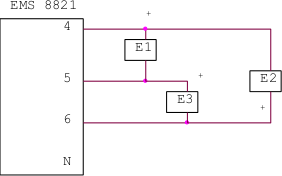
\includegraphics[width=.8\textwidth]{img/circuit_01}
  \caption{Cirucit used to measure line voltages for Part 1}
  \label{fig:circuit_01}
\end{figure}

\begin{figure}[H]
  \centering
  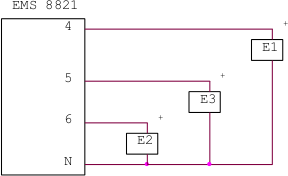
\includegraphics[width=.8\textwidth]{img/circuit_02}
  \caption{Circuit used to measure phase voltages for Part 1}
  \label{fig:circuit_02}
\end{figure}

\begin{figure}[H]
  \centering
  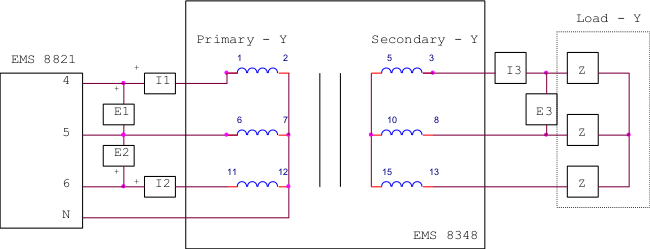
\includegraphics[width=.8\textwidth]{img/circuit_03}
  \caption{Y-Y connected three-phase transformer for Part 2}
  \label{fig:circuit_03}
\end{figure}

\begin{figure}[H]
  \centering
  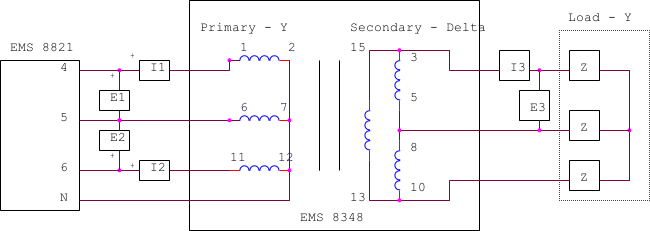
\includegraphics[width=.8\textwidth]{img/circuit_04}
  \caption{Y-$\Delta$ connected three-phase transformer for Part 3}
  \label{fig:circuit_04}
\end{figure}

\end{document}
